\section{Metrics} \label{sec:metrics}

There are many metrics that are standard within the ML community but unconvincing for many parts the geoscience community. 
Specifically, many of these standard scores do not capture the important optimization criteria in the scientific machine learning tasks.
However, there is not consensus within domain-specific communities about the perfect metric which captures every aspect we are interested.
Therefore, we should have a variety of scores from different perspectives to really assess the pros and cons of each method we wish to evaluate thoroughly. 
Below, we outline two sets of scores we use within this framework: skill scores and spectral scores.

\subsection{Skill Scores}

We classify one set of metrics as \textit{skill scores}. 
These are globally averaged metrics which tend to operate within the real space.
Some examples include the root mean squared error (RMSE) and the normalized root mean squared (nRMSE) error.
The RMSE metric can also be calculated w.r.t. the spatial domain, temporal domain or both. 
For example, figure~\ref{fig:oceanbench_psd} showcases the nRMSE calculated only on the spatial domain and visualized for each time step.
%
\begin{align}
    \text{RMSE}: &&\text{RMSE}(\eta,\hat{\eta}) &= ||\eta - \hat{\eta}||_2 \label{eq:RMSE}\\
    % \text{RMSE}_t: &&\text{RMSE}_t(\eta,\hat{\eta}; t) &= ||\eta(t) - \hat{\eta}(t)||_2 \label{eq:RMSE_t}\\
    \text{nRMSE}: &&\text{nRMSE}(\eta,\hat{\eta}) &= 1 - \frac{\text{RMSE}(\eta - \hat{\eta})}{\text{RMSE}(\eta)} \label{eq:nRMSE}
\end{align}
%
However, we are not limited to just the standard MSE metrics.
We can easily incorporate more higher-order statistics like the Centered Kernel Alignment (CKA)~\cite{METRICSCKA} or information theory metrics like mutual information (MI)~\cite{METRICSITRBIG,METRICSITRBIG2}.
In addition, we could also utilize the same metrics in the frequency domain as is done in~\citep{PDEBench}.

\subsection{Spectral Scores}

Another class of scores that we use in \texttt{OceanBench} are the \textit{spectral scores}. These scores are calculated within the spectral space via the wavenumber power spectral density (PSD). 
This provides a spatial-scale-dependent metric which is useful for identifying the largest and smallest scales that were resolved by the reconstruction map. 
In general, we use these to measure the expected energy at different spatiotemporal scales and we can also construct custom score functions which gives us a summary statistic for how well we reconstructed certain scales.
%
\begin{align}
    \text{PSD}: &&\text{PSD}(\eta) &= \sum_{k_{min}}^{k_{max}}\|\mathcal{\mathcal{F}(\eta)}\|^2\label{psd}\\
    \text{PSD}_{score}: &&\text{PSD}_{score}(\eta,\hat{\eta}) &= 1 - \frac{\text{PSD}(\eta - \hat{\eta})}{\text{PSD}(\eta)} \label{eq:psd_score}
\end{align}
%
where $\mathcal{F}$ is the Fast Fourier Transformation (FFT). 
In our application, there are various ways to construct the PSD which depend on the FFT transformation.
We denote the \textit{space-time PSD} as $\lambda_\mathbf{x}$ which does the 2D FFT in the longitude and time direction, then takes the average over the latitude.
We denote the \textit{space-time PSD} as $\lambda_\mathbf{t}$ which does the 2D FFT in the longitude and latitude direction, then takes the average over the time.
We denote the \textit{isotropic PSD} as $\lambda_r$ which assumes a radial relationship in the spatial domain and then averages over the temporal domain.
Lastly, we denote the standard PSD score as $\lambda_a$ which is the 1D FFT over a prescribed distance along the satellite track; this is what is done for the OSE NADIR experiment.
We recognize that the FFT configurations are limited due to their global treatment of the spectral domain and we need more specialized metrics to handle the local scales.
This opens the door to new metrics that handle such cases such as the Wavelet transformation~\cite{METRICSWAVELET}.

\begin{figure}[t!]
\small
\begin{center}
\setlength{\tabcolsep}{1pt}
\begin{tabular}{cccc}
\hspace{3mm} Task OSSE & 
 Task OSSE & 
\hspace{-10mm} Task OSSE & 
\hspace{-10mm}Task OSE \\
\hspace{3mm}  Nadir & 
 Nadir + SWOT & 
\hspace{-10mm} Nadir + SST & 
\hspace{-10mm}Nadir \\
%\vspace{-2mm}
%%%%% SSH %%%%%%%%
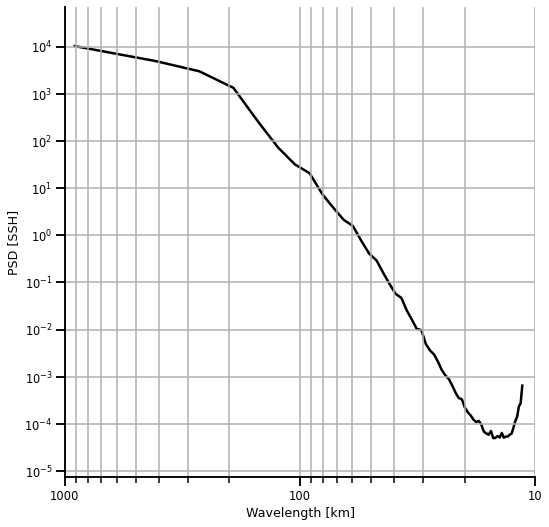
\includegraphics[trim={0 0 0 0},clip, width=3.70cm,height=3.5cm]{00_Oceanbench/content/figures/fourdvarnet_figs/osse_gf_nadir_isotrop.png} &
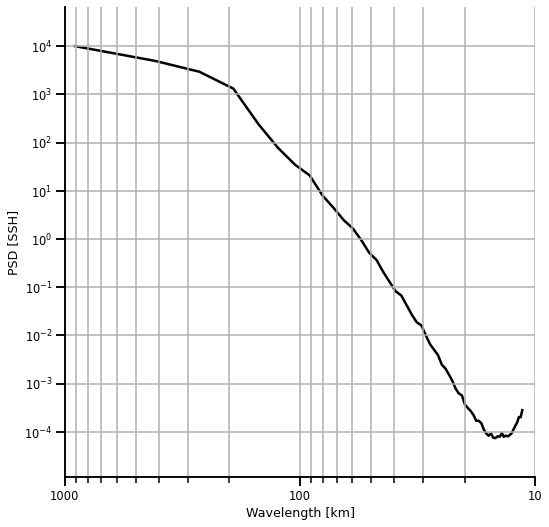
\includegraphics[trim={18mm 0 0 0},clip, width=3.3cm,height=3.5cm]{00_Oceanbench/content/figures/fourdvarnet_figs/osse_gf_nadirswot_isotrop.png} &
\hspace{-5mm}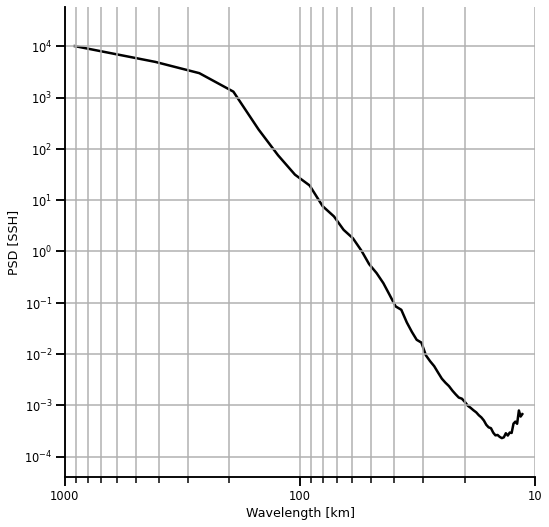
\includegraphics[trim={18mm 0 0 0},clip, width=3.3cm,height=3.5cm]{00_Oceanbench/content/figures/fourdvarnet_figs/osse_gf_nadir_sst_isotrop.png} &
\hspace{-10mm}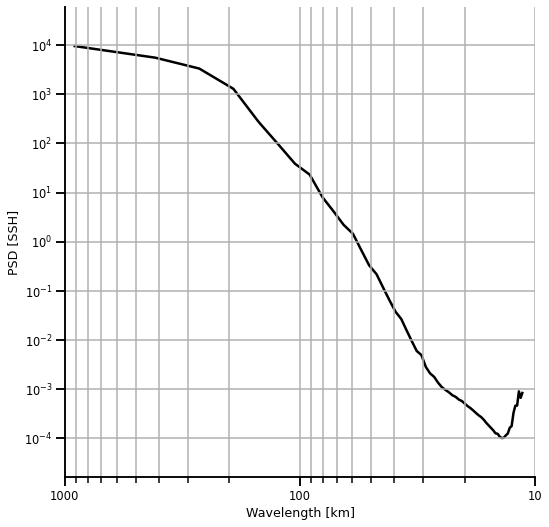
\includegraphics[trim={18mm 0 0 0},clip,width=3.3cm,height=3.5cm]{00_Oceanbench/content/figures/fourdvarnet_figs/ose_gf_isotrop.png} \\
%\vspace{3mm}
%%%%% KINETIC ENERGY %%%%%%%%
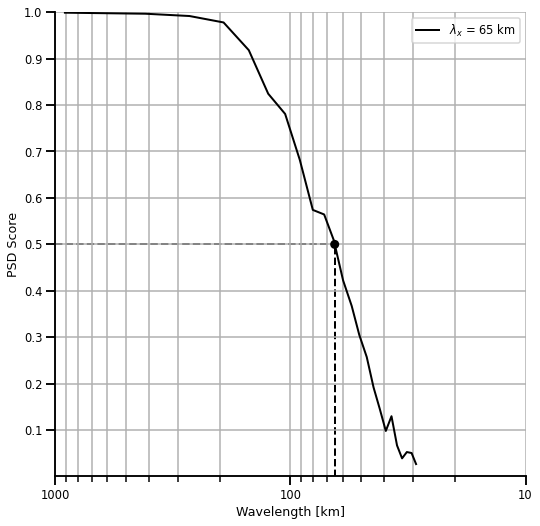
\includegraphics[trim={0 0 0 0}, clip, width=3.70cm,height=3.5cm]{00_Oceanbench/content/figures/fourdvarnet_figs/osse_gf_nadir_1d_psd_score.png} &
\hspace{1mm}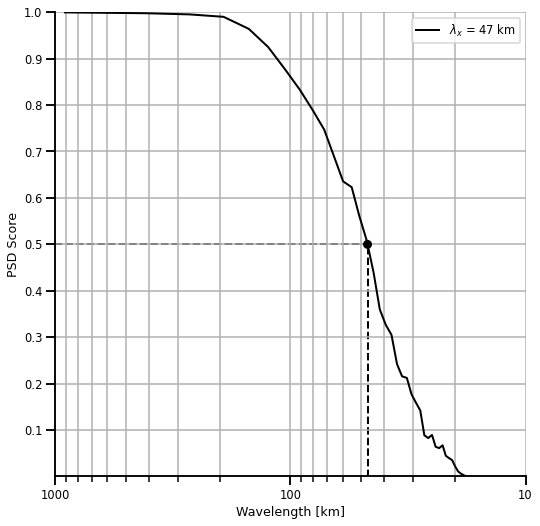
\includegraphics[trim={18mm 0 0 0},clip, width=3.3cm,height=3.5cm]{00_Oceanbench/content/figures/fourdvarnet_figs/osse_gf_nadirswot_1d_psd_score.png} &
\hspace{-4mm}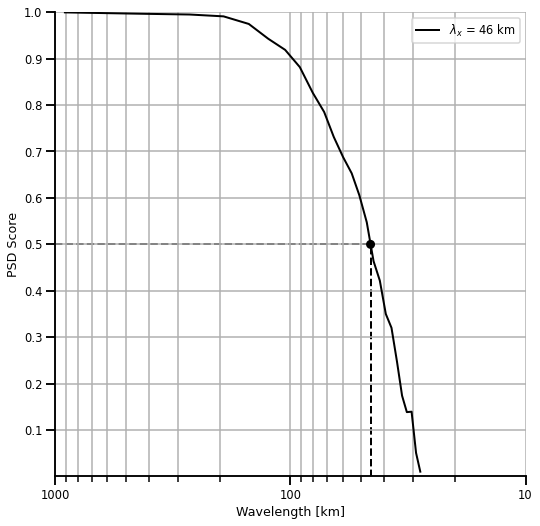
\includegraphics[trim={18mm 0 0 0},clip, width=3.3cm,height=3.5cm]{00_Oceanbench/content/figures/fourdvarnet_figs/osse_gf_nadir_sst_1d_psd_score.png} &
\hspace{-10mm}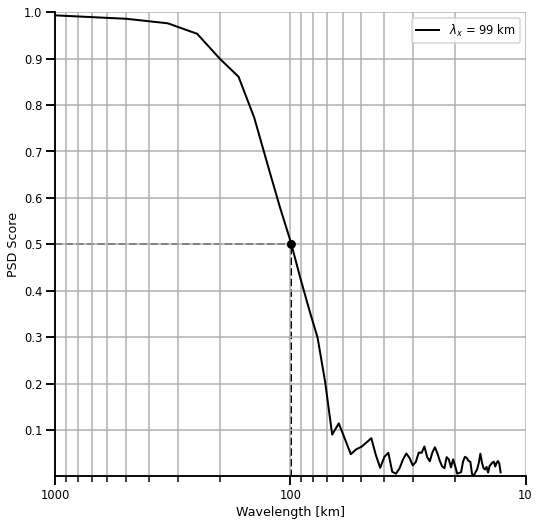
\includegraphics[trim={18mm 0 0 0},clip,width=3.3cm,height=3.5cm]{00_Oceanbench/content/figures/fourdvarnet_figs/ose_gf_1d_psd_score.png} \\
%%%%% RELATIVE VORTICITY %%%%%%%%
\hspace{-4mm}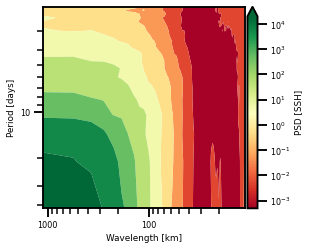
\includegraphics[trim={0 0 23mm 0},clip, width=3.65cm,height=3.5cm]{00_Oceanbench/content/figures/fourdvarnet_figs/osse_gf_nadir_psd_spacetime.png} &
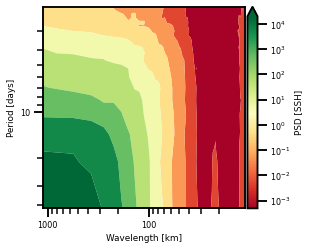
\includegraphics[trim={14mm 0 23mm 0},clip, width=3cm,height=3.5cm]{00_Oceanbench/content/figures/fourdvarnet_figs/osse_gf_nadirswot_psd_spacetime.png} &
\hspace{-5mm}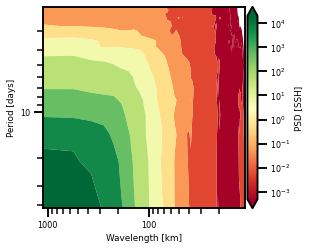
\includegraphics[trim={14mm 0 23mm 0},clip, width=3cm,height=3.5cm]{00_Oceanbench/content/figures/fourdvarnet_figs/osse_gf_nadir_sst_psd_spacetime.png} &
\hspace{-5mm}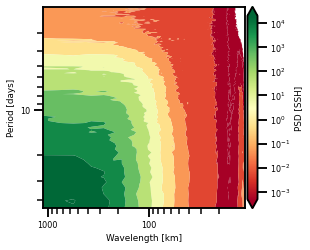
\includegraphics[trim={14mm 0 0 0},clip,width=3.8cm,height=3.5cm]{00_Oceanbench/content/figures/fourdvarnet_figs/ose_gf_psd_spacetime.png} \\
%%%%% STRAIN %%%%%%%%
\hspace{-4mm}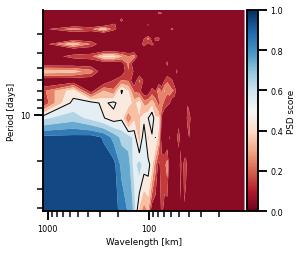
\includegraphics[trim={0 0 23mm 0},clip, width=3.70cm,height=3.5cm]{00_Oceanbench/content/figures/fourdvarnet_figs/osse_gf_nadir_psd_spacetime_score.png} &
\hspace{-2mm}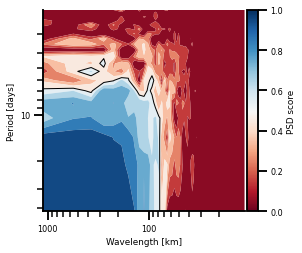
\includegraphics[trim={13mm 0 23mm 0},clip, width=3.1cm,height=3.5cm]{00_Oceanbench/content/figures/fourdvarnet_figs/osse_gf_nadirswot_psd_spacetime_score.png} &
\hspace{1mm}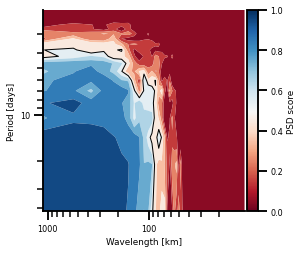
\includegraphics[trim={13mm 0 0 0},clip, width=3.8cm,height=3.5cm]{00_Oceanbench/content/figures/fourdvarnet_figs/osse_gf_nadir_sst_psd_spacetime_score.png} &
 \\
% \vspace{-2mm}
 \hspace{1mm} (a) & \hspace{-5mm} (b) & \hspace{-8mm}(c) & \hspace{-10mm}(d)
\end{tabular}
\vspace{-3mm}
% \caption{Row I - Isotrophic PSD. Row 2 - Isotrophic PSD Score}
\caption{
Power spectrum and associated scores of the 4dVarNet method for each of the four tasks.
The row display in order: (1) the isotropic PSD, (2) the spatial PSD score (using the isotropic PSD for the first three rows and along track PSD for the last row), (3) the space-time PSD, (4) The spacetime PSD score available only in OSSE task.  }

\vspace{-5mm}
\label{fig:oceanbench_psd_4dvarnet}
\end{center}
\end{figure}

% \begin{figure}[h]
% \small
% \begin{center}
% \setlength{\tabcolsep}{1pt}
% \begin{tabular}{cccc}
% \hspace{3mm} NEMO Simulation & 
% \hspace{3mm} MIOST & 
% \hspace{3mm} BFNQG & 
% 4DVarNet \\
% \vspace{-2mm}
% %%%%% SSH %%%%%%%%
% 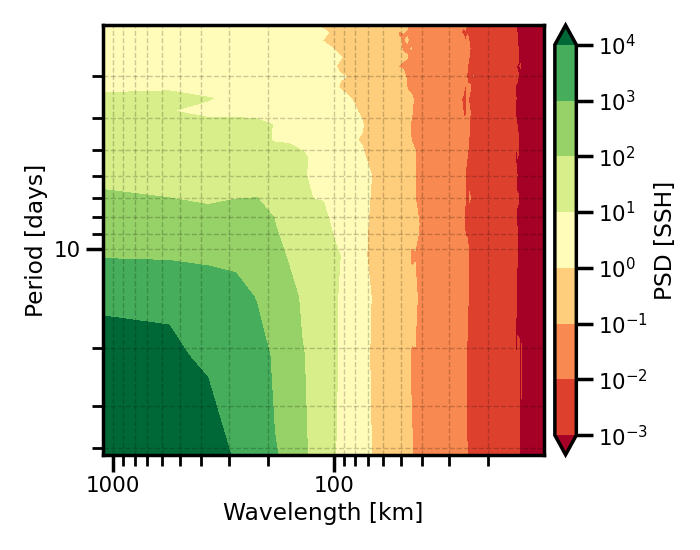
\includegraphics[trim={0 0 38mm 0},clip, width=3.20cm,height=3cm]{content/figures/psd_spacetime/dc20a/nadir4/dc20a_psd_spacetime_nemo_nadir4_ssh.png} &
% 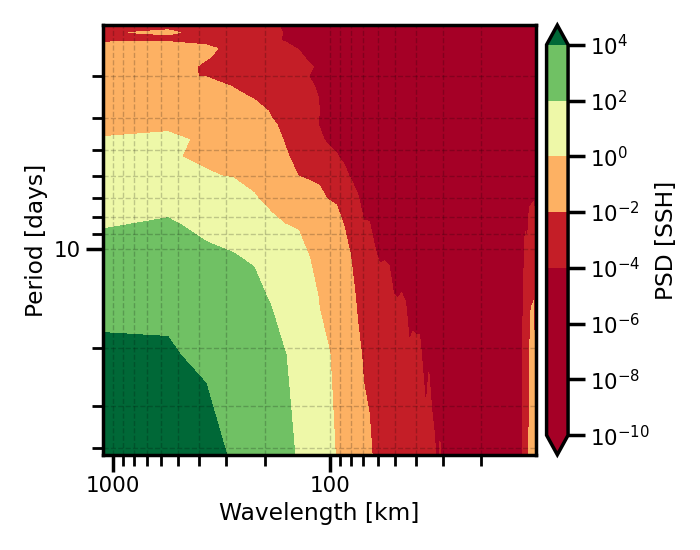
\includegraphics[trim={0 0 40mm 0},clip, width=3.2cm,height=3cm]{content/figures/psd_spacetime/dc20a/nadir4/dc20a_psd_spacetime_miost_nadir4_ssh.png} &
% 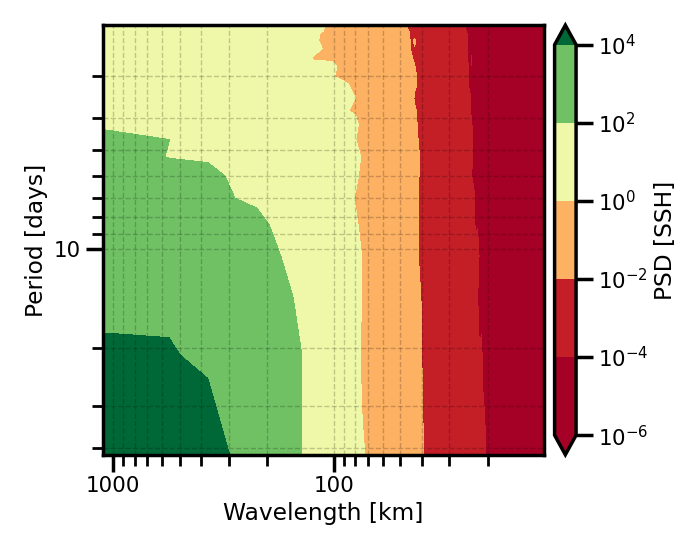
\includegraphics[trim={0 0 38mm 0},clip, width=3.2cm,height=3cm]{content/figures/psd_spacetime/dc20a/nadir4/dc20a_psd_spacetime_bfnqg_nadir4_ssh.png} &
% 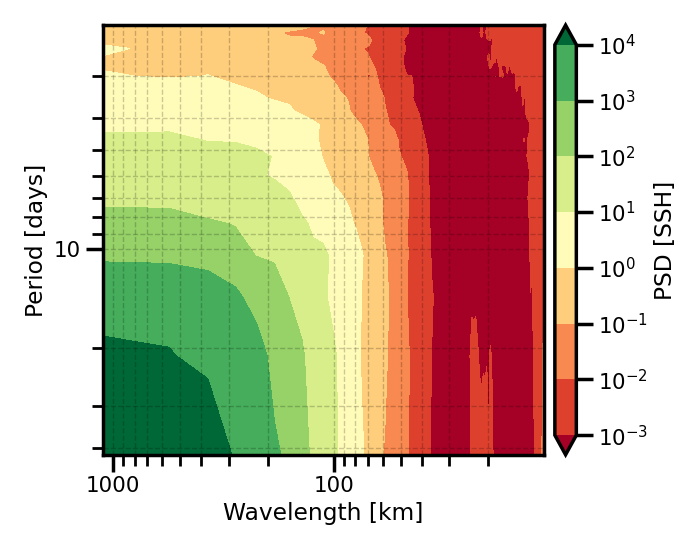
\includegraphics[width=4.0cm,height=3cm]{content/figures/psd_spacetime/dc20a/nadir4/dc20a_psd_spacetime_4dvarnet_nadir4_ssh.png} \\
% \end{tabular}
% % \vspace{-3mm}
% % \caption{Row I - Isotrophic PSD. Row 2 - Isotrophic PSD Score}
% \caption{The space-time power spectrum decomposition.}
% % \vspace{-5mm}
% \label{fig:appendix_psd_spacetime_NADIR}
% \end{center}
% \end{figure}


% \begin{figure}[h]
% \small
% \begin{center}
% \setlength{\tabcolsep}{1pt}
% \begin{tabular}{cccc}
% \hspace{3mm} DUACS & 
% \hspace{3mm} MIOST & 
% \hspace{3mm} BFNQG & 
% 4DVarNet \\
% % \vspace{-2mm}
% %%%%% SSH %%%%%%%%
% 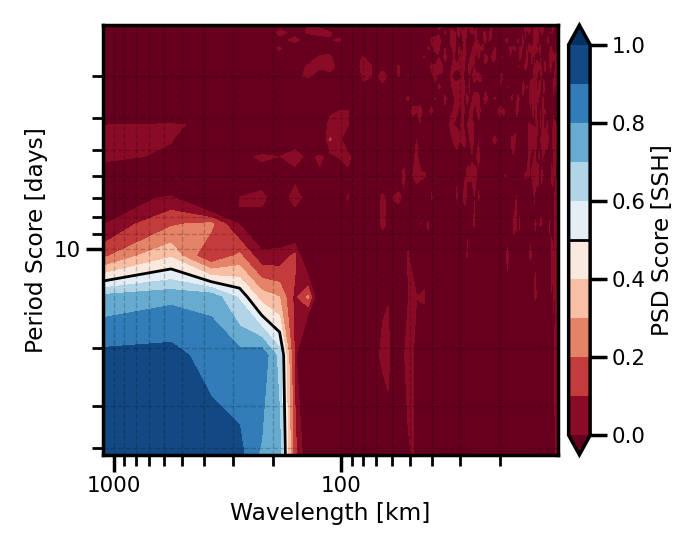
\includegraphics[trim={0 0 38mm 0},clip, width=3.20cm,height=3cm]{content/figures/psd_spacetime/dc20a/nadir4/dc20a_psd_spacetime_score_duacs_nadir4_ssh.png} &
% 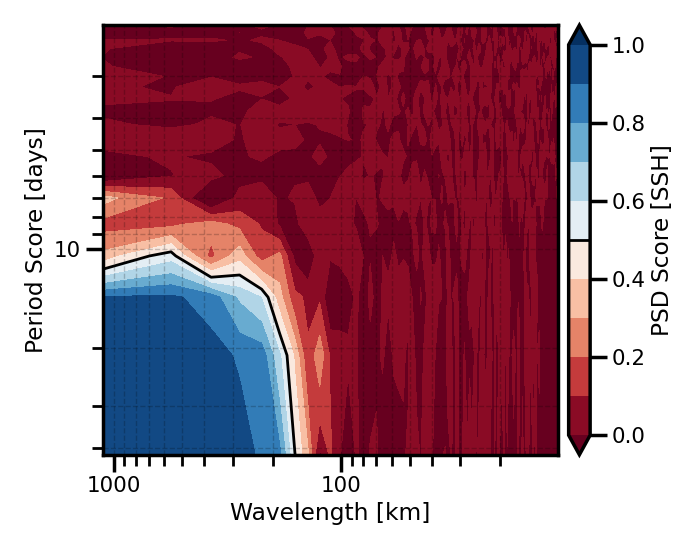
\includegraphics[trim={0 0 40mm 0},clip, width=3.2cm,height=3cm]{content/figures/psd_spacetime/dc20a/nadir4/dc20a_psd_spacetime_score_miost_nadir4_ssh.png} &
% 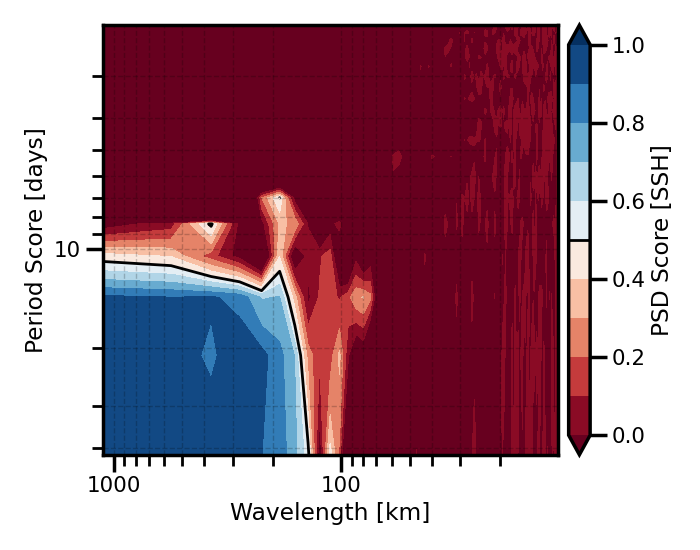
\includegraphics[trim={0 0 38mm 0},clip, width=3.2cm,height=3cm]{content/figures/psd_spacetime/dc20a/nadir4/dc20a_psd_spacetime_score_bfnqg_nadir4_ssh.png} &
% 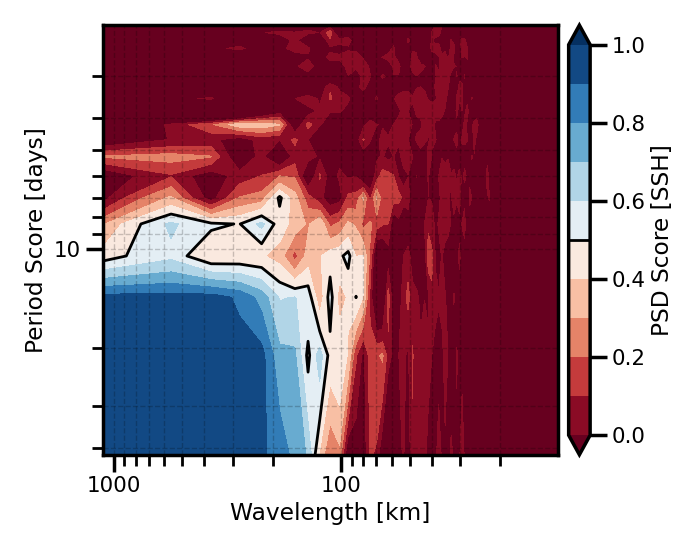
\includegraphics[width=4.0cm,height=3cm]{content/figures/psd_spacetime/dc20a/nadir4/dc20a_psd_spacetime_score_4dvarnet_nadir4_ssh.png} \\
% \end{tabular}
% % \caption{Row I - Isotrophic PSD. Row 2 - Isotrophic PSD Score}
% \caption{The space-time power spectrum score decomposition.}
% % \vspace{-5mm}
% \label{fig:appendix_psd_score_spacetime_NADIR}
% \end{center}
% \end{figure}